\chapter{Designing Change-based Persistence for Models}
\label{ch:change_based_model_persistence}

This chapter presents an illustration of persisting models in change-based format, its requirements, and the design of its implementation. Some potential benefits and novel capabilities as well the challenges of using change-based format for model persistence are also highlighted in this chapter. This chapter also introduces a running example to help explain the approaches proposed in this study.

\section{Introduction}
\label{Introduction}

The concept of change-based persistence that has been presented in the literature review has to be translated into an implementation in a modelling framework context so that it can be applied for model persistence. In order to gain all the benefits of change-based persistence, an implementation that can save and load a model in change-based persistence has to be developed first. The implementation should be able to capture all relevant changes of a model and persist them into a persistence file, as well as to de-serialise changes from the file and (re)execute them in order to (re)construct the model. This research has developed a prototype of such tool, and it has been designed to work with EMF models and metamodels.  

Before going deeper into how the change-based persistence is implemented, this chapter introduces a running to explain the solutions proposed in this study as well as to explain how model differencing and conflict detection are performed in existing tools, such as in EMF Compare \cite{emfcompare2018developer} and EMF Store \cite{emfstore2019what}. It illustrates cases where existing tools and the proposed approaches of this study can be different in identifying differences and detecting conflicts.

The rest of this chapter is structured as follows. Section \ref{sec:running_example_1} introduces the running example.
Sections \ref{sec:proposed_approach} and \ref{sec:requirements} overview the proposed approach and its requirements.
Section \ref{sec:prototype_implementation} discusses the prototype 
implementation on top of the Eclipse Modelling Framework. 
The potential benefits and novel capabilities, as well as the challenges 
of change-based model persistence, are presented in 
Section \ref{sec:benefits_and_novel_capabilities}. Section \ref{sec:conclusions_3} concludes this chapter.

%To reap the benefits of Model-Based Software Engineering in the context 
%of large and complex systems in collaborative environment, the ability to identify differences and conflicts between versions of large models as they evolve is essential. Current traditional, state-based model comparison only deliver limited performance benefits due to slow and imprecise model differencing and conflict detection which can be a bottleneck for real-world software development projects. The research introduced in this thesis aims at enabling high-performance model differencing and conflict detection through 
%change-based model persistence. That is, instead of persisting snapshots 
%of the states of models, this research proposes persisting models on their change history. The proposed approach has the potential to deliver faster model differencing and conflict detection as well as a wide range of other benefits and novel capabilities.

\section{Running Example}
\label{sec:running_example_1}

\begin{figure}[ht]
  \centering
  \begin{subfigure}[t]{0.45\linewidth}
    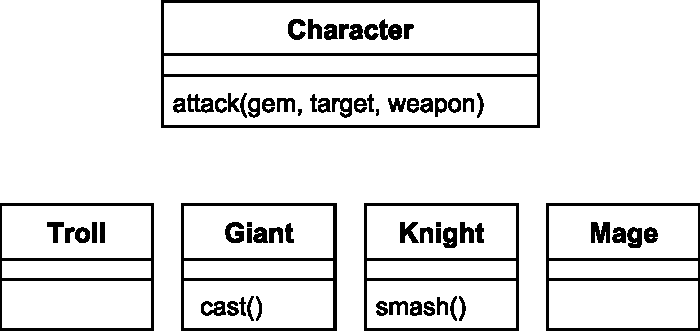
\includegraphics[width=\linewidth]{class_diagram_origin}
    \caption{original version (Jane's version)}
    \label{fig:class_diagram_origin}
  \end{subfigure}
  \\
  \begin{subfigure}[t]{0.45\linewidth}
    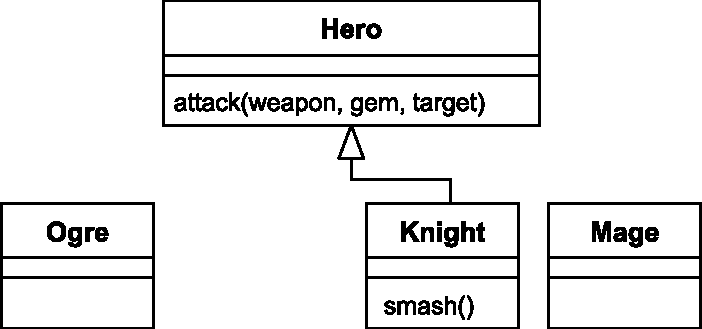
\includegraphics[width=\linewidth]{class_diagram_left}
    \caption{left version (Bob's version)}
    \label{fig:class_diagram_left}
  \end{subfigure}
  \hfill
  \begin{subfigure}[t]{0.45\linewidth}
    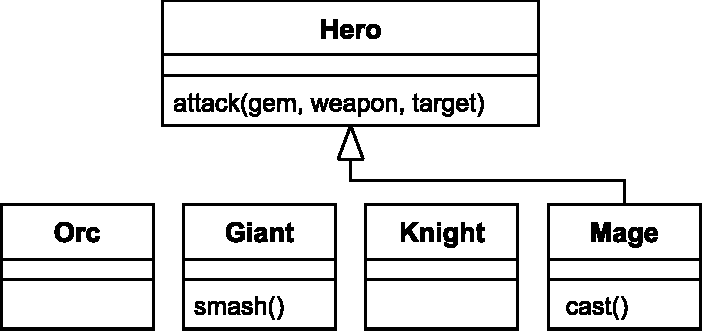
\includegraphics[width=\linewidth]{class_diagram_right}
    \caption{right version (Alice's version)}
    \label{fig:class_diagram_right}
  \end{subfigure}
  \caption{Three class diagrams of a Role Playing Game.}
  \label{fig:class_diagram_rpg}
\end{figure}

Let's say that there is a project to develop a Role Playing Game (RPG), and UML2 class diagram is used to model the game (it is important to note that the the class diagram's metamodel has been modified so that a class can only have one superclass as in Java; this has an implication on explaining how EMF Store detects conflict later on in Chapter \ref{ch:conflict_detection}). Jane, as the technical leader, set up the initial model (Figure \ref{fig:class_diagram_origin}). Jane produced classes for Character and 4 specific types of character, but did not determine the relationships among these. She then assigned Bob and Alice to continue the work. Working separately on this original model, Bob and Alice made different decisions about subclassing, renamed some character types, and, in Bob’s case, deleted one character type, producing the models in Figures \ref{fig:class_diagram_left} and \ref{fig:class_diagram_right} respectively. The models are still incomplete, and it is desirable to merge the designs at this point. However, the revisions have introduced inconsistencies that we need to identify, and resolve, before creating a new definitive model from the two new versions. Finding the differences and conflicts between these two versions are discussed in Chapters \ref{ch:model_differencing} and \ref{ch:conflict_detection}. Persisting these models in the standard XMI \cite{omg2018xmi} format produces three files as shown in Listings \ref{lst:xmimodel_origin}, \ref{lst:xmimodel_left}, and \ref{lst:xmimodel_right}. 

\begin{wrapfigure}[23]{r}{0.53\textwidth}
\vspace{-32pt}
\begin{lstlisting}[style=eol,caption={Change-based representation of the original version in Figure \ref{fig:class_diagram_origin}.},label=lst:cbp_origin]
session "Jane-01"
create character type Class
set character.name from null to "Character" 
create attack type Operation
set attack.name from null to "attack" 
add attack to character.operations at 0
create gem type Parameter
set gem.name from null to "gem" 
add gem to attack.parameters at 0
create target type Parameter
set target.name from null to "target" 
add target to attack.parameters at 1
create weapon type Parameter
set weapon.name from null to "weapon" 
add weapon to attack.parameters at 2
create troll type Class
set troll.name from null to "Troll" 
create giant type class
set giant.name from null to "Giant"
create cast type Operation
set cast.name from null to "smash"
add cast to giant.operations at 0
create knight type Class
set knight.name from null to "Knight"
create smash type Operation
set smash.name from null to "smash"
add smash to knight.operations at 0
create mage type Class
set mage.name from null to "Mage" 
\end{lstlisting}
\end{wrapfigure}

Let's say Jane, Bob, and Alice also implement the change-based proposed in this paper. So, instead of only persisting the snapshots of models, they also persist the complete history of changes of models, in the form of atomic change events, into change-based model persistence. As an example, the complete history of changes made by Jane to construct the original version in Figure \ref{fig:class_diagram_origin} is also persisted in a change-based model representation as displayed in Listing \ref{lst:cbp_origin}. The change events made by Bob is displayed in Listing \ref{lst:cbp_left}. In the implementation, his change events are appended to Jane's original change events. Thus, the change events that represent Bob's version (Figure \ref{fig:class_diagram_left}) consists of the original change events and the change events (Listing \ref{lst:cbp_left}) made by him. The change events that represents Alice's version (Figure \ref{fig:class_diagram_right}) is presented in Listing \ref{lst:cbp_right}. 



Let's say the complete scenario that produces the models in Figures \ref{fig:class_diagram_origin}, \ref{fig:class_diagram_left}, and \ref{fig:class_diagram_right} as wells Listings \ref{lst:cbp_origin}, \ref{lst:cbp_left}, and \ref{lst:cbp_right} occured according to the following story. Jane, as the technical leader, set up the initial model. The records of events during setting up the initial is recorded in the change-based persistence in Listing \ref{lst:cbp_origin}. She created a class \textsf{Character} that contains an operation \textsf{attack} with three parameters: \textsf{gem}, \textsf{target}, and \textsf{weapon} (lines 2-15). She also created four other classes; \textsf{Troll} (lines 16-17), \textsf{Giant} (lines 18-22), \textsf{Knight} (lines 23-27), and \textsf{Mage} (lines 28-29). She then pushed her work to a change-based version control system. If her work is visualised in state-based format, the model looks like in Figure \ref{fig:class_diagram_origin}.

\vspace{-20pt}
\begin{lstlisting}[firstnumber=30,style=eol,escapechar=|,caption={The appended events made by Bob to produce the left version in Figure \ref{fig:class_diagram_left} (left version).},label=lst:cbp_left]
session "Bob-01"|\label{line:cbp_left_30}|
create leftGen type Generalization|\label{line:cbp_left_31}|
set leftGen.general to character|\label{line:cbp_left_32}|
set troll.generalization to leftGen|\label{line:cbp_left_33}|
set character.name from "Character" to "Hero"|\label{line:cbp_left_34}|
unset troll.generalization from leftGen to null composite l1|\label{line:cbp_left_35}|
set knight.generalization to leftGen composite l1|\label{line:cbp_left_36}|
move target in attack.parameters from 1 to 2|\label{line:cbp_left_37}|
unset cast.name from "cast" to null composite l2|\label{line:cbp_left_38}|
remove cast from giant.operations at 0 composite l2|\label{line:cbp_left_39}|
delete cast composite l2|\label{line:cbp_left_40}|
unset giant.name from "Giant" to null composite l2|\label{line:cbp_left_41}|
delete giant composite l2|\label{line:cbp_left_42}|
set troll.name from "Troll" to "Ogre"|\label{line:cbp_left_43}|
\end{lstlisting}

\vspace{-20pt}
\begin{lstlisting}[firstnumber=30,style=eol,escapechar=|,caption={The appended events made by Alice to produce the right version in Figure \ref{fig:class_diagram_right} (right version).},label=lst:cbp_right]
session "Alice-01"|\label{line:cbp_right_30}|
move target in attack.parameters from 1 to 0|\label{line:cbp_right_31}|
remove smash from knight.operations at 0 composite r1|\label{line:cbp_right_32}|
add smash to giant.operations at 0 composite r1|\label{line:cbp_right_33}|
remove cast from giant.operations at 1 composite r2|\label{line:cbp_right_34}|
add cast to mage.operations at 0 composite r2|\label{line:cbp_right_35}|
create rightGen type Generalization|\label{line:cbp_right_36}|
set rightGen.general to character|\label{line:cbp_right_37}|
set troll.generalization to rightGen|\label{line:cbp_right_38}|
set character.name from "Character" to "Hero"|\label{line:cbp_right_39}|
unset troll.generalization from rightGen to null composite r3|\label{line:cbp_right_40}|
set mage.generalization to rightGen composite r3|\label{line:cbp_right_41}|
set troll.name from "Troll" to "Orc"|\label{line:cbp_right_42}|
\end{lstlisting}

She then assigned this work to Bob and Alice. Both of them checked out this project to their own machine. Alice then started to continue the model. She then moved parameter \textsf{target} to the first place in operation \textsf{attack}'s parameters, because she thought it was more intuitive for programmers to think about the \textsf{target} first than the rest parameters (List. \ref{lst:cbp_right}, line 31). She also moved operation \textsf{smash} from class \textsf{Knight} to class \textsf{Giant} and operation \textsf{cast} from class \textsf{Giant} to class \textsf{Mage} as they are more reasonable to belong to their new classes (lines 32-35). Alice also created a generalisation relationship with id \textsf{rightGen} from class \textsf{Troll} to class \textsf{Character} (36-39). Bob also did the same thing except that his generalisation came with id \textsf{leftGen} (List. \ref{lst:cbp_left}, line 31-33). 

Later on, Jane then informed them that she wanted all good characters should be derived from a general, hero-like class, and the enemy should be the Orcs not Trolls. She also instructed that Bob should focus on developing class \textsf{Knight} and Alice on class \textsf{Mage}. In consequence, Alice then changed the name of class \textsf{Character} from ``Character'' to ``Hero'' (the id of class \textsf{Hero} is still \textsf{character}) (line 39). Again, Bob did the same thing. He also changed the name of class \textsf{Character} from ``Character'' to ``Hero'' (line 34). Instead of creating a new generalisation relationship, both of them preferred to move the generalisation relationships that they had created to their assigned classes. Alice moved generalisation \textsf{rightGen} from class \textsf{Troll} to class \textsf{Mage} (lines 40-41), and Bob move generalisation \textsf{leftGen} from class \textsf{Troll} to class \textsf{Knight} (lines 35-36). Bob also moved parameter \textsf{target} in operation \textsf{attack} to the last index as he thought setting target as the last parameter was intuitive (line 37), and deleted the class {Giant}, and unfortunately, he deleted class \text{Giant} accidentally (lines 38-42). The class diagrams of Bob and Alice's models are visualised in Figures \ref{fig:class_diagram_left} and \ref{fig:class_diagram_right} respectively. Lastly, Alice changed the \textsf{name} of class \textsf{Troll} to ``Orc'' (line 42) while Bob changed it to ``Ogre'' (line 43).  


\section{Proposed Approach}
\label{sec:proposed_approach}
As mentioned before, this research aims to enable high-performance model differencing and conflict detection. Instead of persisting the snapshots of the states of models (which is what virtually all modelling tools and frameworks currently do), this work proposes persisting models in their change history.

To illustrate the proposed approach, Listing \ref{lst:xmimodel_left} shows a state-based representation of the model of Figure \ref{fig:class_diagram_left} in (simplified) XMI, and Listing \ref{lst:cbp_left} shows the proposed equivalent change-based representation of the same model. Instead of a snapshot of the state of the model, the representation of Listing \ref{lst:cbp_left} captures the complete sequence of change events (create/set/add/move/remove/delete) that were performed on the model since its creation, organised in editing sessions. There are two editing sessions in the case of this model: one in Listing \ref{lst:cbp_left} and another in Listing \ref{lst:cbp_origin}. In the actual implementation, change events in Listing \ref{lst:cbp_left} are appended to a file that is a copy of Listing \ref{lst:cbp_origin}. Listing \ref{lst:cbp_left} only shows the appended change events, while Listing \ref{lst:cbp_left_full} shows the complete change events. Replaying these changes, the change events in Listing \ref{lst:cbp_origin} first and then followed by the change events in Listing \ref{lst:cbp_left}, produces the same state as the one captured in Listing \ref{lst:xmimodel_left}. Thus, we can conclude that the proposed change-based representation carries at least as much information as the state-based representation. 

Such a representation is particularly suitable to identify recent changes of the model since the last version. For example, if we can identify that changes recorded for the previous version is up to right before the editing session \textsf{Bob-01} (lines 1-29) of the model, it can readily identify the changes that have been made to the model since then (i.e. in session \textsf{Bob-01} -- lines 30-43) instead of having to rediscover them through expensive state-based model differencing.
For the sake of readability, the format of change-based persistence presented in Listing \ref{lst:cbp_left_full} is a simplified version. The real format is XML-like format, and it would be something similar to the change-based file in Listing \ref{lst:class_diagram_left_cbpfile} in Appendix \ref{sec:examples_of_cbp}. For example, change event \textsf{session "Jane-01"} is persisted as:

\textsf{<session id="Jane-01" time="20190923181841687GMT"/>} 

and \textsf{set character.name from null to "Character"} is persisted as:

\textsf{<set-eattribute eclass="Class" name="name" target="character"><old-value literal = null/><value literal="Character"/></set-eattribute>}.

In Listing \ref{lst:cbp_left_full}, we also introduce composite events -- lines with keyword \textsf{composite} -- that represent composite change events. 
Composite change events are events that should be treated as one composition -- identified with the same composite id. 
For example, moving an element from a container to another container is a composite event since it consists of two change events: 
removing/unsetting the element from its source container and adding/setting it to its target container (lines 40-41 Listing \ref{lst:cbp_left_full}). 

\section{Requirements}
\label{sec:requirements}
From the literature review and the text-based change summaries in the above listings, a number of requirements have been gathered as guidance for designing the implementation of the change-based persistence.
\begin{enumerate}
  \item[R1] The implementation should be able to listen and collect change events when a model is modified.
  \item[R2] It should conform to model and metamodel infrastructure of Eclipse Modeling Framework.
  \item[R3] A change event should contain necessary information, such as change event type (add, remove, delete, create, set, unset, composite), element (class and id), feature (name and type), value (literal or object), and index (from and to), so that when replaying them orderly an equivalent model can be constructed.
  \item[R4] The implementation should be able to append change events into a change-based model file as well as to (re)load them from the file by replaying all the change events.
\end{enumerate}
 
\section{Prototype Implementation}
\label{sec:prototype_implementation}
Based on the requirements, this work has implemented a prototype \cite{epsilonlabs2019emfcbp} of the change-based model persistence format -- the prototype is named EMF CBP -- using the notification facilities provided by the Eclipse Modelling Framework. In the implementation, the prototype uses a subclass of EMF's \textsf{EContentAdapter} (\textsf{ChangeEventAdapter}) so that it can receive and record \textsf{Notification} events produced by the framework for every model-element-feature level change. Using these EMF's classes enable the prototype to address requirements R1 and R2.

\begin{figure}[th]
    \centering
    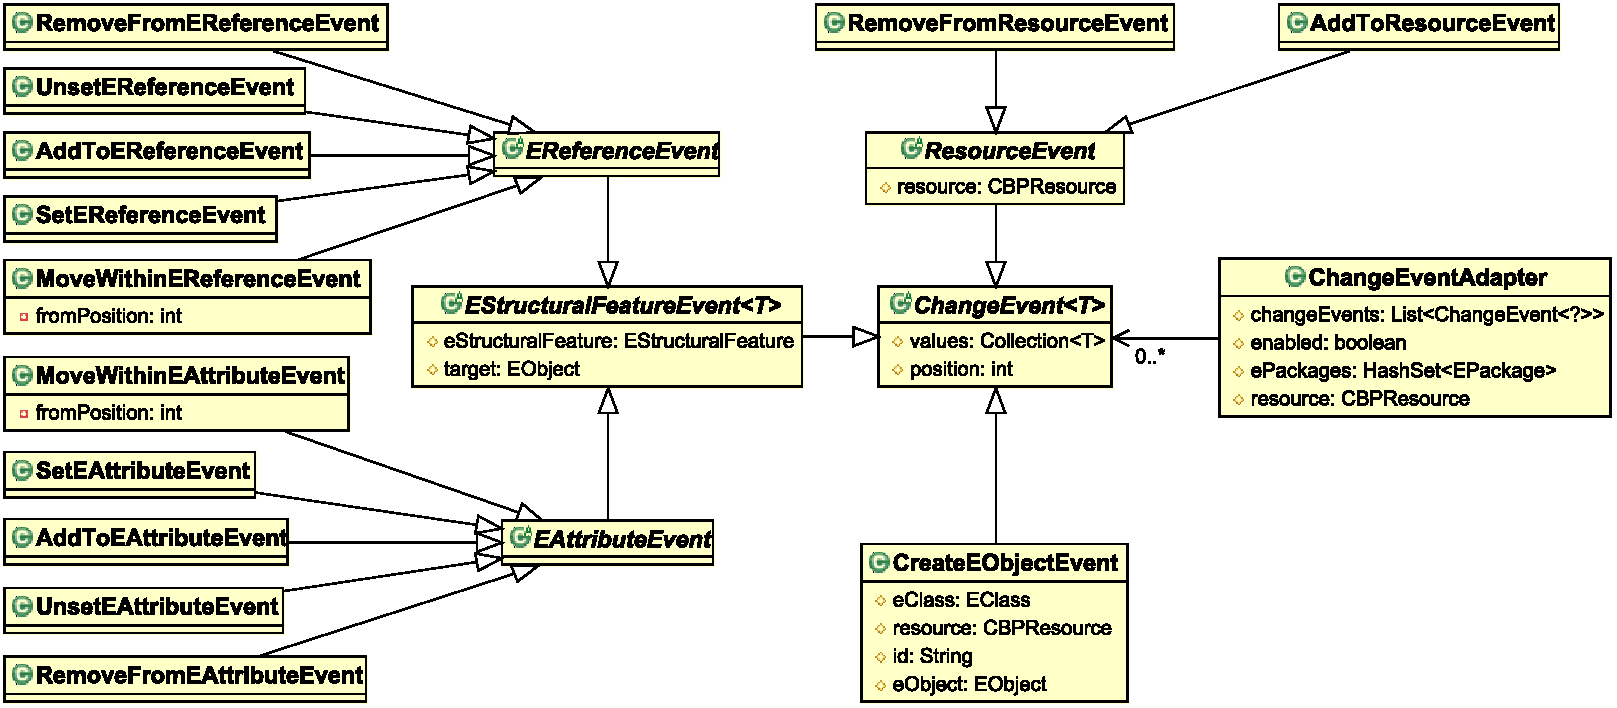
\includegraphics[width=\linewidth]{events}
    \caption{Event classes to represent changes of models.}
    \label{fig:events}
\end{figure}

Since not all change events are relevant to change-based persistence (e.g. EMF also produces change notifications when listeners/adapted are added/removed from the model), this work has defined a set of event classes to represent change events of interest. The event classes are depicted in Figure \ref{fig:events} as subclasses of the \textsf{ChangeEvent} abstract class. In this way, we can define all shared attributes and methods among change events  only at the \textsf{ChangeEvent} class, and perform polymorphism when replaying different kinds of change events.

EMF has dedicated classes to express the graph structure of a model, such as \textsf{EFeature} can be \textsf{EReference} or \textsf{EAttribute}, it can have single value or multi values (e.g., Integer, String), the value(s) of \textsf{EFeature} can be type of \textsf{EObject} or primitive, the \textsf{EReference} can be type of containment or non-containment, and etc. These characteristics drive the design of the prototype to have different subclasses of \textsf{ChangeEvent} also decide which attributes and methods should be defined in the class. 

The \textsf{ChangeEvent} class has a multi-valued \textsf{values} attribute which can accommodate both single-valued (e.g. set/add) or multi-valued events (e.g. addAll/removeAll). \textsf{ChangeEvent} can also accommodate different types of values, such as \textsf{EObject}s for \textsf{EReferenceEvents}, and primitive values (e.g., Integer, String) for \textsf{EAttributeEvents}. The \textsf{ChangeEvent} class also has a position attribute to hold the index of an \textsf{EObject} or a literal when they are added to a \textsf{Resource}, \textsf{EReference}, or \textsf{EAttribute} with multiple values. Every time an \textsf{EObject} is added to the model, a \textsf{CreateEObjectEvent} and an \textsf{AddToResourceEvent} are recorded. When an EObject is deleted, or moved to a containment \textsf{EReference} deeper in the model, a \textsf{RemoveFromResourceEvent} is recorded. Having these different subclasses of \textsf{ChangeEvent} accommodates the prototype to meet requirements R2 and R3.
\begin{lstlisting}[style=java,caption={Simplified Java code to handle notification events.},label=lst:javacode]
public class ChangeEventAdapter extends EContentAdapter {
...
@override
public void notifyChanged(Notification n) {
    ...
    switch (n.getEventType()) {
    ... // other events
    case Notification.UNSET: {
        if (n.getNotifier() instanceof EObject) {
            EStructuralFeature feature = (EStructuralFeature) n.getFeature();
            if (feature instanceof EAttribute) {
                event = new UnsetEAttributeEvent();
            } else if (feature instanceof EReference) {
                event = new UnsetEReferenceEvent();
            }
        } break;
    } 
    ... // other events
\end{lstlisting}	

The \textsf{ChangeEventAdapter} receives EMF change notifications in its \textsf{notifyChanged()} method and filters and transforms them into appropriate change events. As an example of how notifications are filtered and transformed, Listing \ref{lst:javacode} shows how the prototype handles \textsf{Notification.UNSET} events based on the type of the changed feature i.e. an \textsf{UnsetEAttributeEvent} is instantiated if the feature of the notifier is an \textsf{EAttribute}, or an \textsf{UnsetEReferenceEvent}  is created if the notifier is an \textsf{EReference}. The transformed instances are then stored into a list of events in \textsf{ChangeEventAdapter} (\textsf{changeEvents}) for persistence. 

To integrate seamlessly with the EMF framework and to eventually support multiple concrete change-based serialisation formats (e.g. XML-formatted representation for readability and binary for performance/size), the prototype implemented \textsf{CBPResource} abstract class, that extends EMF's built-in \textsf{ResourceImpl} class. The role of the abstract class is to encapsulate all change recording functionality while the role of its concrete subclasses is to implement serialisation and de-serialisation. To save a model, \textsf{CBPXMLResourceImpl} persists changes in a line-based format where every change is serialised as a single-line XML document. In this way, when a model changes, the prototype can append the new changes to the end of the model file without needing to serialise the entire model again. To load a model, \textsf{CBPXMLResourceImpl} treated the persisted file as an XML document. It de-serialised every line in the document as a change event and then re-execute it to re-construct the model. Having the ability to save and load a model change-based persistence means that the prototype has meet the requirement R4.  The prototype has also implemented a \textsf{CBPXMLResourceFactory} class that extends EMF's \textsf{ResourceFactoryImpl}, as the factory class for change-based models. Figure \ref{fig:resources} shows the relationships between these classes.

\begin{figure}[th]
    \centering
    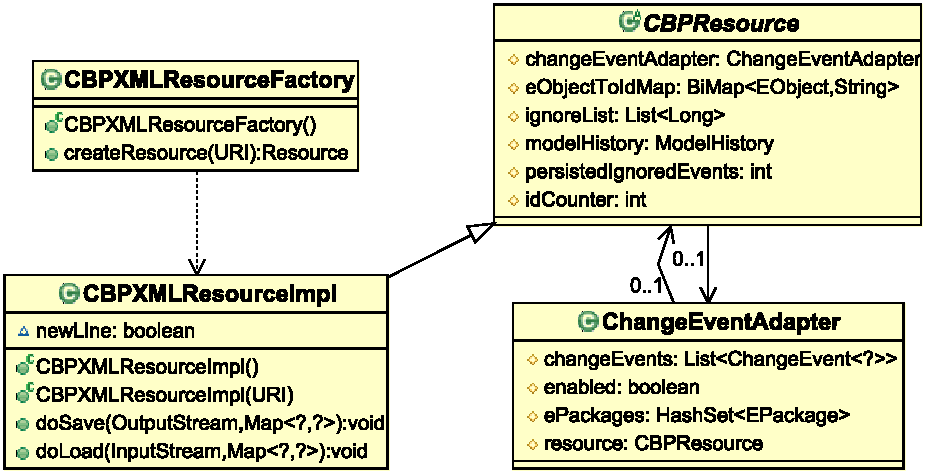
\includegraphics[width=0.75\linewidth]{resources}
    \caption{Factory, resources, and ChangeEventAdapter classes.}
    \label{fig:resources}
\end{figure}

Listing \ref{lst:javacode_resource} shows an example how to use the prototype in a Java code. Lines 1-8 demonstrate how to initialise and save a model using the prototype. First, the code creates an instance of \textsf{CBPResource}, \textsf{cbpResource}, using \textsf{CBPXMLResourceFactory} and specify its file as \textsf{helloworld.cbpxml} using \textsf{URI}. The code than executes method \textsf{startNewSession} of \textsf{cbpResource}. This method adds a change event to indicate the start of editing session as depicted at line 1 in Listings \ref{lst:cbp_origin} and \ref{lst:class_diagram_left_cbpfile}.
The code then uses \textsf{UMLFactory} to create an element, \textsf{model}, of UML2's \textsf{Model}. The code adds element \textsf{model} into \textsf{cbpResource} and set the name to ``Hello World''. The code then saves the model in change-based format using method \textsf{save} and then unload \textsf{cbpResource}. Lines 9-12 demonstrate how to replay (load) the model that previously has been saved and then print the name of the first element in \textsf{cbpResource} which is expected to print ``Hello World'' text.
\begin{lstlisting}[style=java,caption={An example how to use \textsf{CBPResource} in Java code.},label=lst:javacode_resource]
/* initialise, save, and unload */
CBPResource cbpResource = (CBPResource) (new CBPXMLResourceFactory()).createResource(URI.createFileURI("helloworld.cbpxml"));
cbpResource.startNewSession("Initial");
Model model = UMLFactory.eINSTANCE.createModel();
cbpResource.getContents().add(model);
model.setName("Hello World");
cbpResource.save(null);
cbpResource.unload();

/* load and print */
cbpResource.load(null);
model = (Model) cbpResource.getContents().get(0);
System.out.println(model.getName()); // expected output: "Hello World"
\end{lstlisting}

\section{Benefits and Novel Capabilities}
\label{sec:benefits_and_novel_capabilities}
This section highlights some of the benefits, and the novel capabilities of the change based persistence prototype can deliver, compared to the currently prevalent state-based representations, some of which are discussed below.

\begin{itemize}
\item With appropriate tool support, modellers will be able to ``replay" (part of) the change history of a model (e.g. to understand design decisions made by other developers, for training purposes). In state-based approaches, this can be partly achieved if models are stored in a version-control repository (e.g. Git). However, the granularity would only be at the commit level.
\item By analysing models serialised in the proposed representation, modelling language and tool vendors will be able to develop deeper insights into how modellers actually use these languages/tools in practice and utilise this information to guide the evolution of the language/tool. An early work for this case can be seen in \cite{polack2019towards}.
\item By attaching additional information to each session (e.g. the id of the developer, references to external documents/URLs), sequences of changes can be traced back to the developer that made them, or to requirements/bug reports that triggered them.
\item Persisting changes to large models after an editing session will be significantly faster compared to serialising the entire state of the model, as only changes made during the session will need to be appended to the model file. The evaluation of this benefit can be found in \cite{yohannis2018towards,DBLP:conf/models/YohannisRPK18} or Chapters \ref{ch:optimised_loading} and \ref{ch:hybrid_model_persistence} of this thesis.
\item The performance and precision of model differencing and conflict detection can be substantially improved, particularly for large models with shared editing histories. The evaluation of this benefit can be found in \cite{yohannis2019efficient} or Chapters \ref{ch:model_differencing} and \ref{ch:conflict_detection} of this thesis.
\item Using a text file to persist changes of a model allows common text-oriented version controls, such as Git and SVN, to be potentially used for model versioning, which are not supported by EMF Store -- an existing implementation of change-based persistence of EMF models -- that uses its own mechanism to version models.
\end{itemize}

\section{Challenges}
\label{sec:challenges}
This section highlights the challenges that comes when adopting change-based persistence. As has been mentioned in the literature review, change-based persistence also comes with a number of challenges, such as (1) loading overhead and (2) fast-growing model files, which can hold back the delivery of its potential benefits. Addressing this challenges surely facilitates its adoption.

For the first challenge, while, as discussed above, persisting changes to large models is expected to be much faster and resource-efficient compared to state-based approaches, loading models into memory by naively replaying the entire change history is expected to have a significant overhead. This work has addressed this challenge by proposing two solutions that reduces the cost of change-based model loading. The first solution is by recording and ignoring events -- events that are later overridden or cancelled out by other events -- The solution can be found in Chapter \ref{ch:optimised_loading} and \cite{yohannis2018towards}. The second solution is by proposing a hybrid model persistence format, that is using change-based and state-based persistence side-by-side. In this solution, changes applied to a model are persisted into both change-based and state-based representation, but for loading, the model is loaded from the stated-based persistence thus it avoids replaying the change events. This solution is discussed in \ref{ch:hybrid_model_persistence} and \cite{DBLP:conf/models/YohannisRPK18}. 

For the second challenge -- the fast-growing model files challenge, persisting models in a change-based format means that model files will keep growing in size during their evolution significantly faster than their state-based counterparts. This challenge has not been addressed in this research and naturally is part of future work. Nevertheless, the solutions that this research recommends are one can proposes sound change-compression operations (e.g. remove older/unused information) that can be used to reduce the size of a model in a controlled way or develops a compact textual format that will minimise the amount of space required to record a change (a textual line-separated format is desirable to maintain compatibility with file-based version control systems).   

\section{Conclusions}
\label{sec:conclusions_3}
Through persisting models' change history, this research aims at enabling high-performance model differencing and conflict detection in collaborative development settings. The concept of change-based persistence has to be translated into an implementation in a modelling framework context so that it can be applied for model persistence. 

In this chapter, a running example has been introduced. This example is used throughout this thesis to explain the solutions proposed in this study. A prototype of a change-based persistence format also has been presented, including its requirements as well as the design of the implementation to meet the requirements. Some potential benefits and novel capabilities that a change-based persistence can contribute and the challenges that might restrain delivering them also have been presented.   

This chapter also has addressed partially the first research question of this study (RQ1), \textbf{How can models be effectively persisted in a change-based format?}. In order to persist models in change-based format, a prototype has been developed. It captures relevant notifications returned by the notification facilities provided by EMF every time as change is applied to an EMF model. It then transforms the notifications into different classes of change events representing different types of changes (e.g., set, unset, add, remove, move, create, and delete) that conform to the model and metamodel infrastructure of EMF. Every captured change event is then persisted by appending it into an XML-like-formatted file when the model is saved. The model can be (re)loaded by de-serialising the file and (re)executing all the persisted change events -- replaying the historical construction of the model.


